\documentclass[10pt,a4paper,oneside]{book}

\begin{document}

\chapter{Laboratory Instructions}

This laboratory is divided into three different experiments. In the first part, you will measure the point spread function (PSF) and estimate the localization precision of single fluorescent molecules. You will do this using fluorescent beads deposited onto a glass coverslip.

In the second experiment, you will perform STORM imaging of tubulin. Tubulin is the protein that makes up microtubules, one of the filaments comprising the cytoskeleton. In this experiment, tubulin in COS7 cells has been labeled with the fluorescent dye AlexaFluor 647. You will image these markers and reconstruct the microtubule network in the cell.

In the third part, you will perform STORM imaging of mitochondria, also using AlexaFluor 647 as a fluorescent marker for the mitochondrial outer membrane in COS7 cells. Mitochondria are tube-like organelles that produce energy for the cell. Since they are effectively 2D structures, they will require a different set of imaging parameters than the tubulin, which is effectively 1D.

\section{Safety}

\fbox{
    \parbox{\textwidth}{\textbf{WARNING} The buffers used in SMLM contain highly toxic chemicals. Always follow proper laboratory safety procedures and wear the proper personal protective equipment. Please alert a teaching assistant immediately if any of the buffer touches you.}
}\newline

\noindent\fbox{
    \parbox{\textwidth}{\textbf{WARNING} SMLM imaging requires the use of high-powered lasers. A safety interlock over the objective is in place to avoid accidental exposure. Do not attempt to bypass the interlock.}
}\newline

\section{Description of the Microscope}

The microscope is an Abbelight SAFe 180. It consists of an Olympus IX83 microscope, an Abbelight scanning illumination system, an Oxxius laser engine, a Hamamatsu ORCA-Fusion digital CMOS camera, and other components. Some of these components are labeled in \autoref{fig:microscope} and \autoref{fig:electronics}.

\begin{figure}[ht]
    \centering
    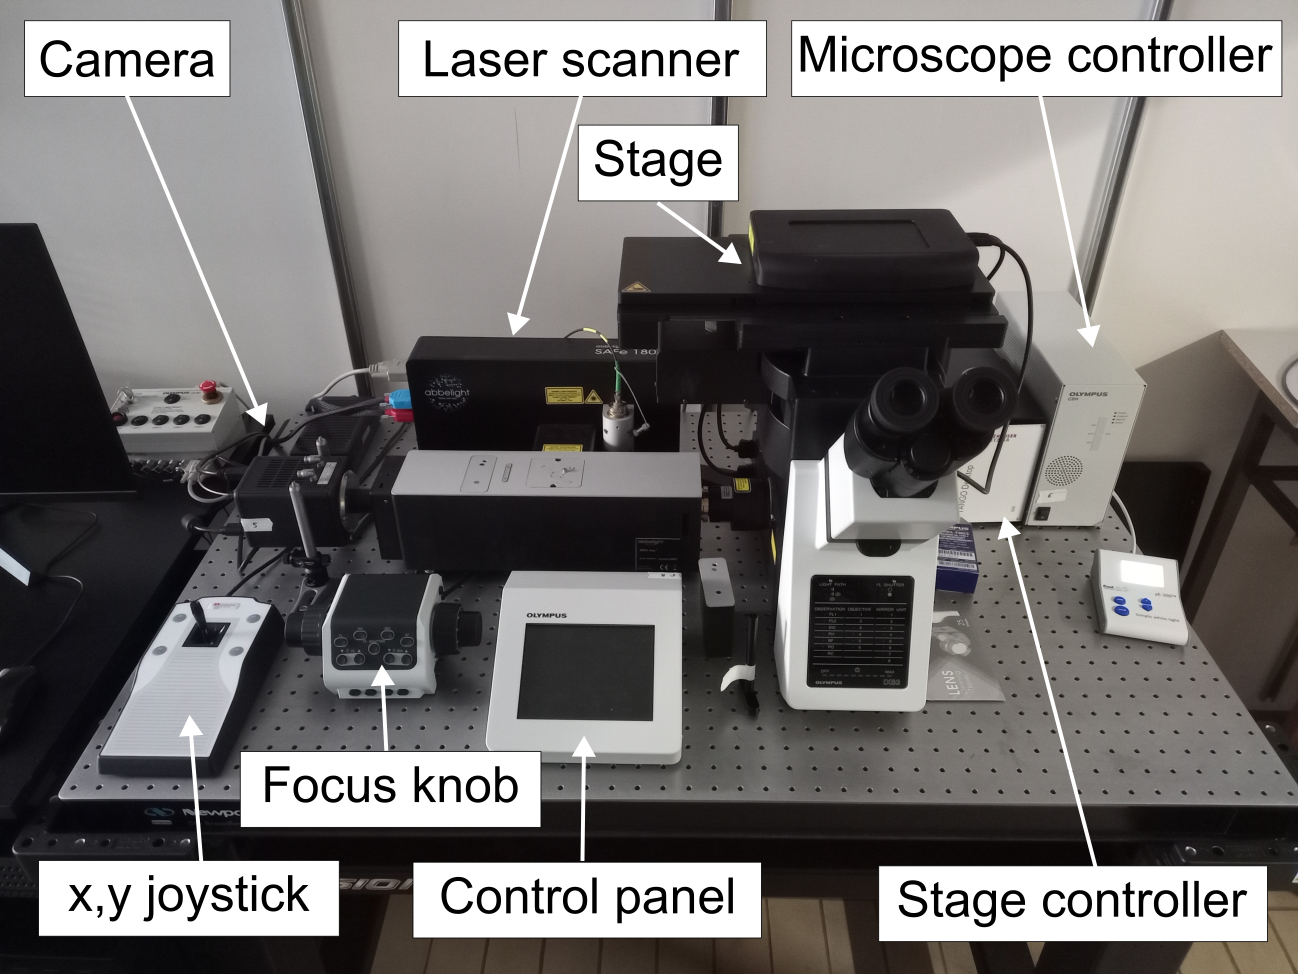
\includegraphics[width=0.75\textwidth]{microscope.png}
    \caption{The primary components of the microscope used in this course.}
    \label{fig:microscope}
\end{figure}

\begin{figure}[ht]
    \centering
    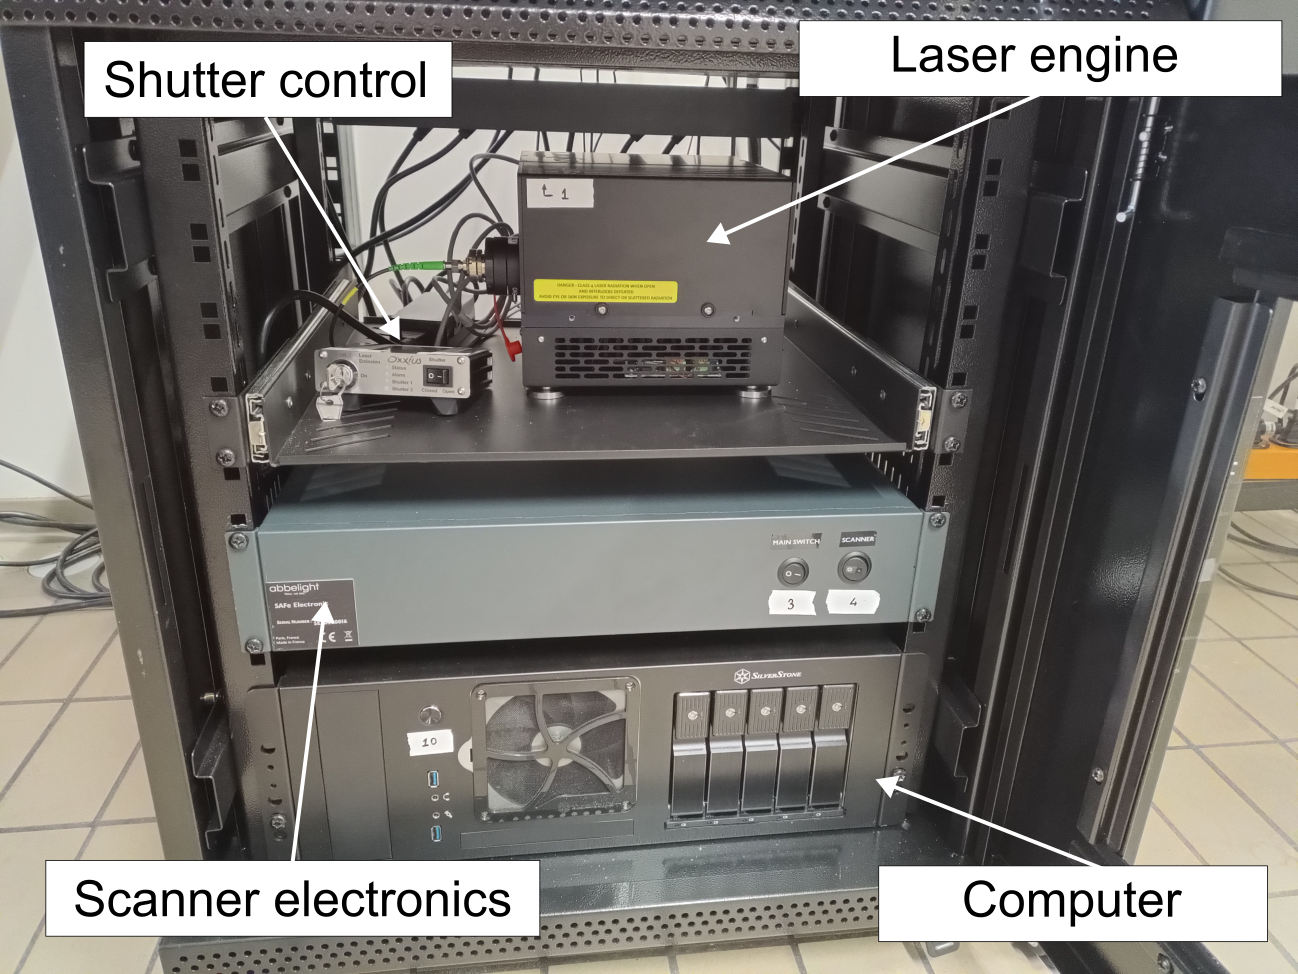
\includegraphics[width=0.75\textwidth]{electronics.png}
    \caption{Electronics and laser source for the microscope.}
    \label{fig:electronics}
\end{figure}

You may learn more about the microscope here: \url{https://www.abbelight.com/solutions/bioimaging-instruments/}.

\section{Materials and Waste}

The following materials are used in this laboratory:

\begin{itemize}
  \item Cell samples on glass coverslips
  \item Abbelight Smart Buffer kits
  \item Gloves
  \item $1000 \, \mu L$ micropipette (blue) and tips
  \item $200 \, \mu L$ micropipette (yellow) and tips
  \item $10 \, \mu L$ micropette (red) and tips
  \item Cavity well slides
  \item Immersion oil
  \item Cleaning tissue
  \item Lens cleaning solvent (ethanol 90% - 99%)
  \item Tweezers
  \item  PBS (1x)
  \item Plastic dishes for mixing paste
\end{itemize}

The following waste is generated in this laboratory and must be disposed of in the proper bin. The following goes in biological waste:

\begin{itemize}
  \item PBS
  \item Cells / coverslips
  \item Used pipette tips
  \item  Gloves
\end{itemize}

Ethanol (EPFL OMoD code: 07 01 04) goes in the bin for alcohols; the used STORM buffer (EPFL OMoD code: 16 05 06) has its own special bin.

\section{Common Procedures}

The following procedures are common to all experiments.

\subsection{Turn On the Microscope}\label{sec:startup}

To turn on the microscope, turn on the following components in this order. There should be pieces of tape with numbers on them and attached to the actual devices to aid you.

\textbf{In the electronics cabinet:}

\begin{enumerate}
    \item Laser engine
    \item Laser safety key on the shutter controller
    \item Scanner electronics: main switch
    \item Scanner electronics: scanner
\end{enumerate}

\textbf{On the optical table:}

\begin{enumerate}
    \item Camera \newline Wait for the status light to turn green before proceeding.
    \item Olympus CBH microscope controller
    \item Maerhaeuser Tango Desktop stage controller
    \item Olympus control panel \newline Wait for the "Start Operation" button to appear, then press it to continue. This can take about one minute.
\end{enumerate}

\textbf{Back in the electronics cabinet:}

\begin{enumerate}
    \item Laser shutter
    \item The computer
\end{enumerate}

\subsection{Mount the Slide onto the Microscope}\label{sec:mount-slide}

\autoref{fig:objective-sample} illustrates how the sample should be mounted onto the microscope for all of the experiments in this course. The side with the sample must face in towards the buffer, and the side of the slide with the coverslip must be closest to the microscope objective.

\begin{figure}[ht]
    \centering
    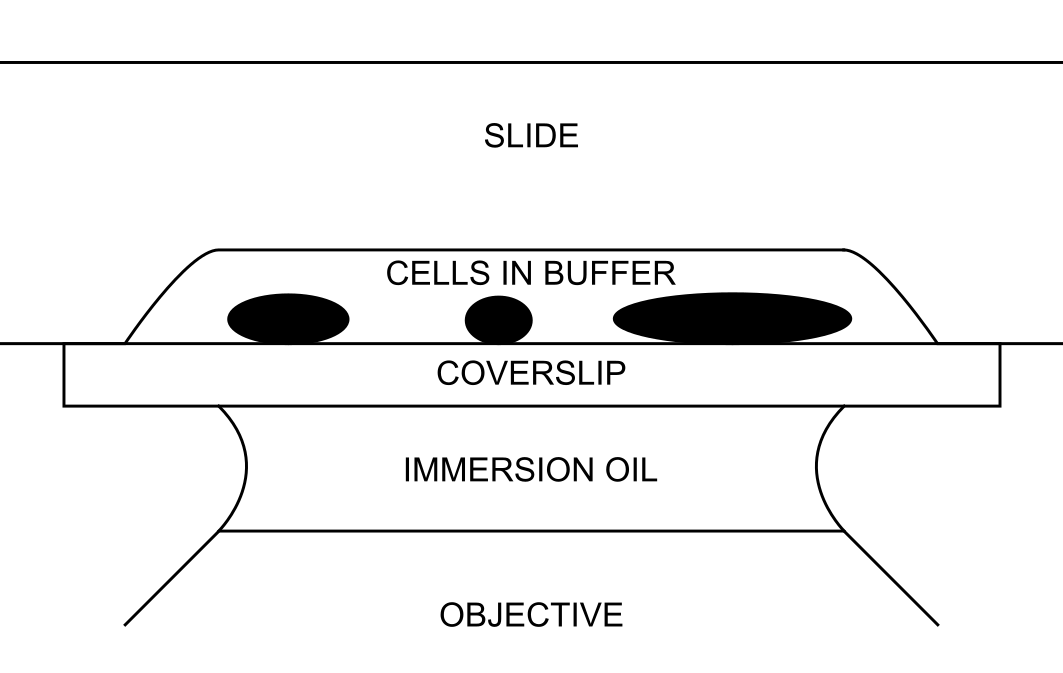
\includegraphics[width=0.75\textwidth]{oil-immersion-objective-with-sample.png}
    \caption{Illustration of the sample/objective space showing the relative positions of the various components and media. This illustration is not to scale!}
    \label{fig:objective-sample}
\end{figure}

Mounting the slide requires only immersion oil.

To mount the slide onto the microscope, first remove the black safety cover over the objective. Place a small drop of immersion oil on top of the objective lens. Only one small drop is necessary! The immersion oil allows light rays at large angles to the microscope axis to enter the objective's aperture. This increases the resolution of the microscope.

Next, turn the focus knob so that the microscope objective is all the way down as indicated by the yellow line in the objective position indicator section of the microscope control panel. Then, place the slide into the sliding black metallic mounts and gently push them together until the slide is secure. Ensure that the coverslip is centered over the objective. Finally, turn the focus knob to raise the objective slowly until it is just touching the oil. You will know when the objective is touching the oil because you can see the oil spreading out underneath the objective. A video that illustrates this effect may be found at \url{https://drive.google.com/file/d/1IC5Azq-raW6_jVSnuBDrSsZ0OsQYxoPK/view?usp=sharing}.

When done, replace the black safety cover over the objective and sample.

\textbf{At this point, continue to the instructions for the specific experiment you are performing, i.e. \autoref{sec:exp1}, \autoref{sec:exp2}, or \autoref{sec:exp3}}.

\subsection{Turn Off the Microscope}

Turn off the components in the opposite order as in \autoref{sec:startup}.

\subsection{Remove Oil From the Objective}\label{sec:remove-oil}

\subsubsection{Materials}

\begin{itemize}
    \item{Ethanol}
    \item{Lens cleaning tissue}
    \item{Tweezers}
\end{itemize}

The oil must be removed from the objective after imaging, and sometimes during imaging if there is dust in the oil. To do this, use lens cleaning solution and lens tissue to clean the objective. The lens tissue should be folded into a small square and wetted with the cleaning solution. In this laboratory, ethanol is used as the solution, though this can vary with objective manufacturers. Avoid touching the area of the tissue that you will use to clean the objective. After wetting, gently wipe the objective with the lens tissue, slowly moving the tissue across the objective in one direction. Repeat the process if oil remains.

A video demonstration on cleaning objectives may be found at \url{https://www.youtube.com/watch?v=Tz4Dy5D6kdw}.

\section{Experiment 1 - Measure the PSF and Localization Precision}\label{sec:exp1}

In this experiment, you will measure the point spread function (PSF) of the microscope and the localization precision. The PSF is a measure of the resolution of the microscope. The localization precision is a measure of the precision with which you can determine position of a single fluorescent molecule.

\subsection{Materials}

\begin{itemize}
    \item{Bead sample}
    \item{Immersion oil}
    \item{Lens cleaning products (see \autoref{sec:remove-oil})}
\end{itemize}

\subsection{Procedure}

\subsubsection{Setup the Microscope Configuration}

The bead sample is comprised of 0.1 $\mu m$ diameter fluorescent beads attached to a glass coverslip. Their small size makes them good approximations to single molecules. The bead sample is provided to you in this lab.

After mounting the bead sample and making contact with the immersion oil (\autoref{sec:mount-slide}), you should start the imaging software which is called \textbf{NEO Live Imaging}. You will see a screen like the one in \autoref{fig:liveimaging-startup}.

\begin{figure}[ht]
    \centering
    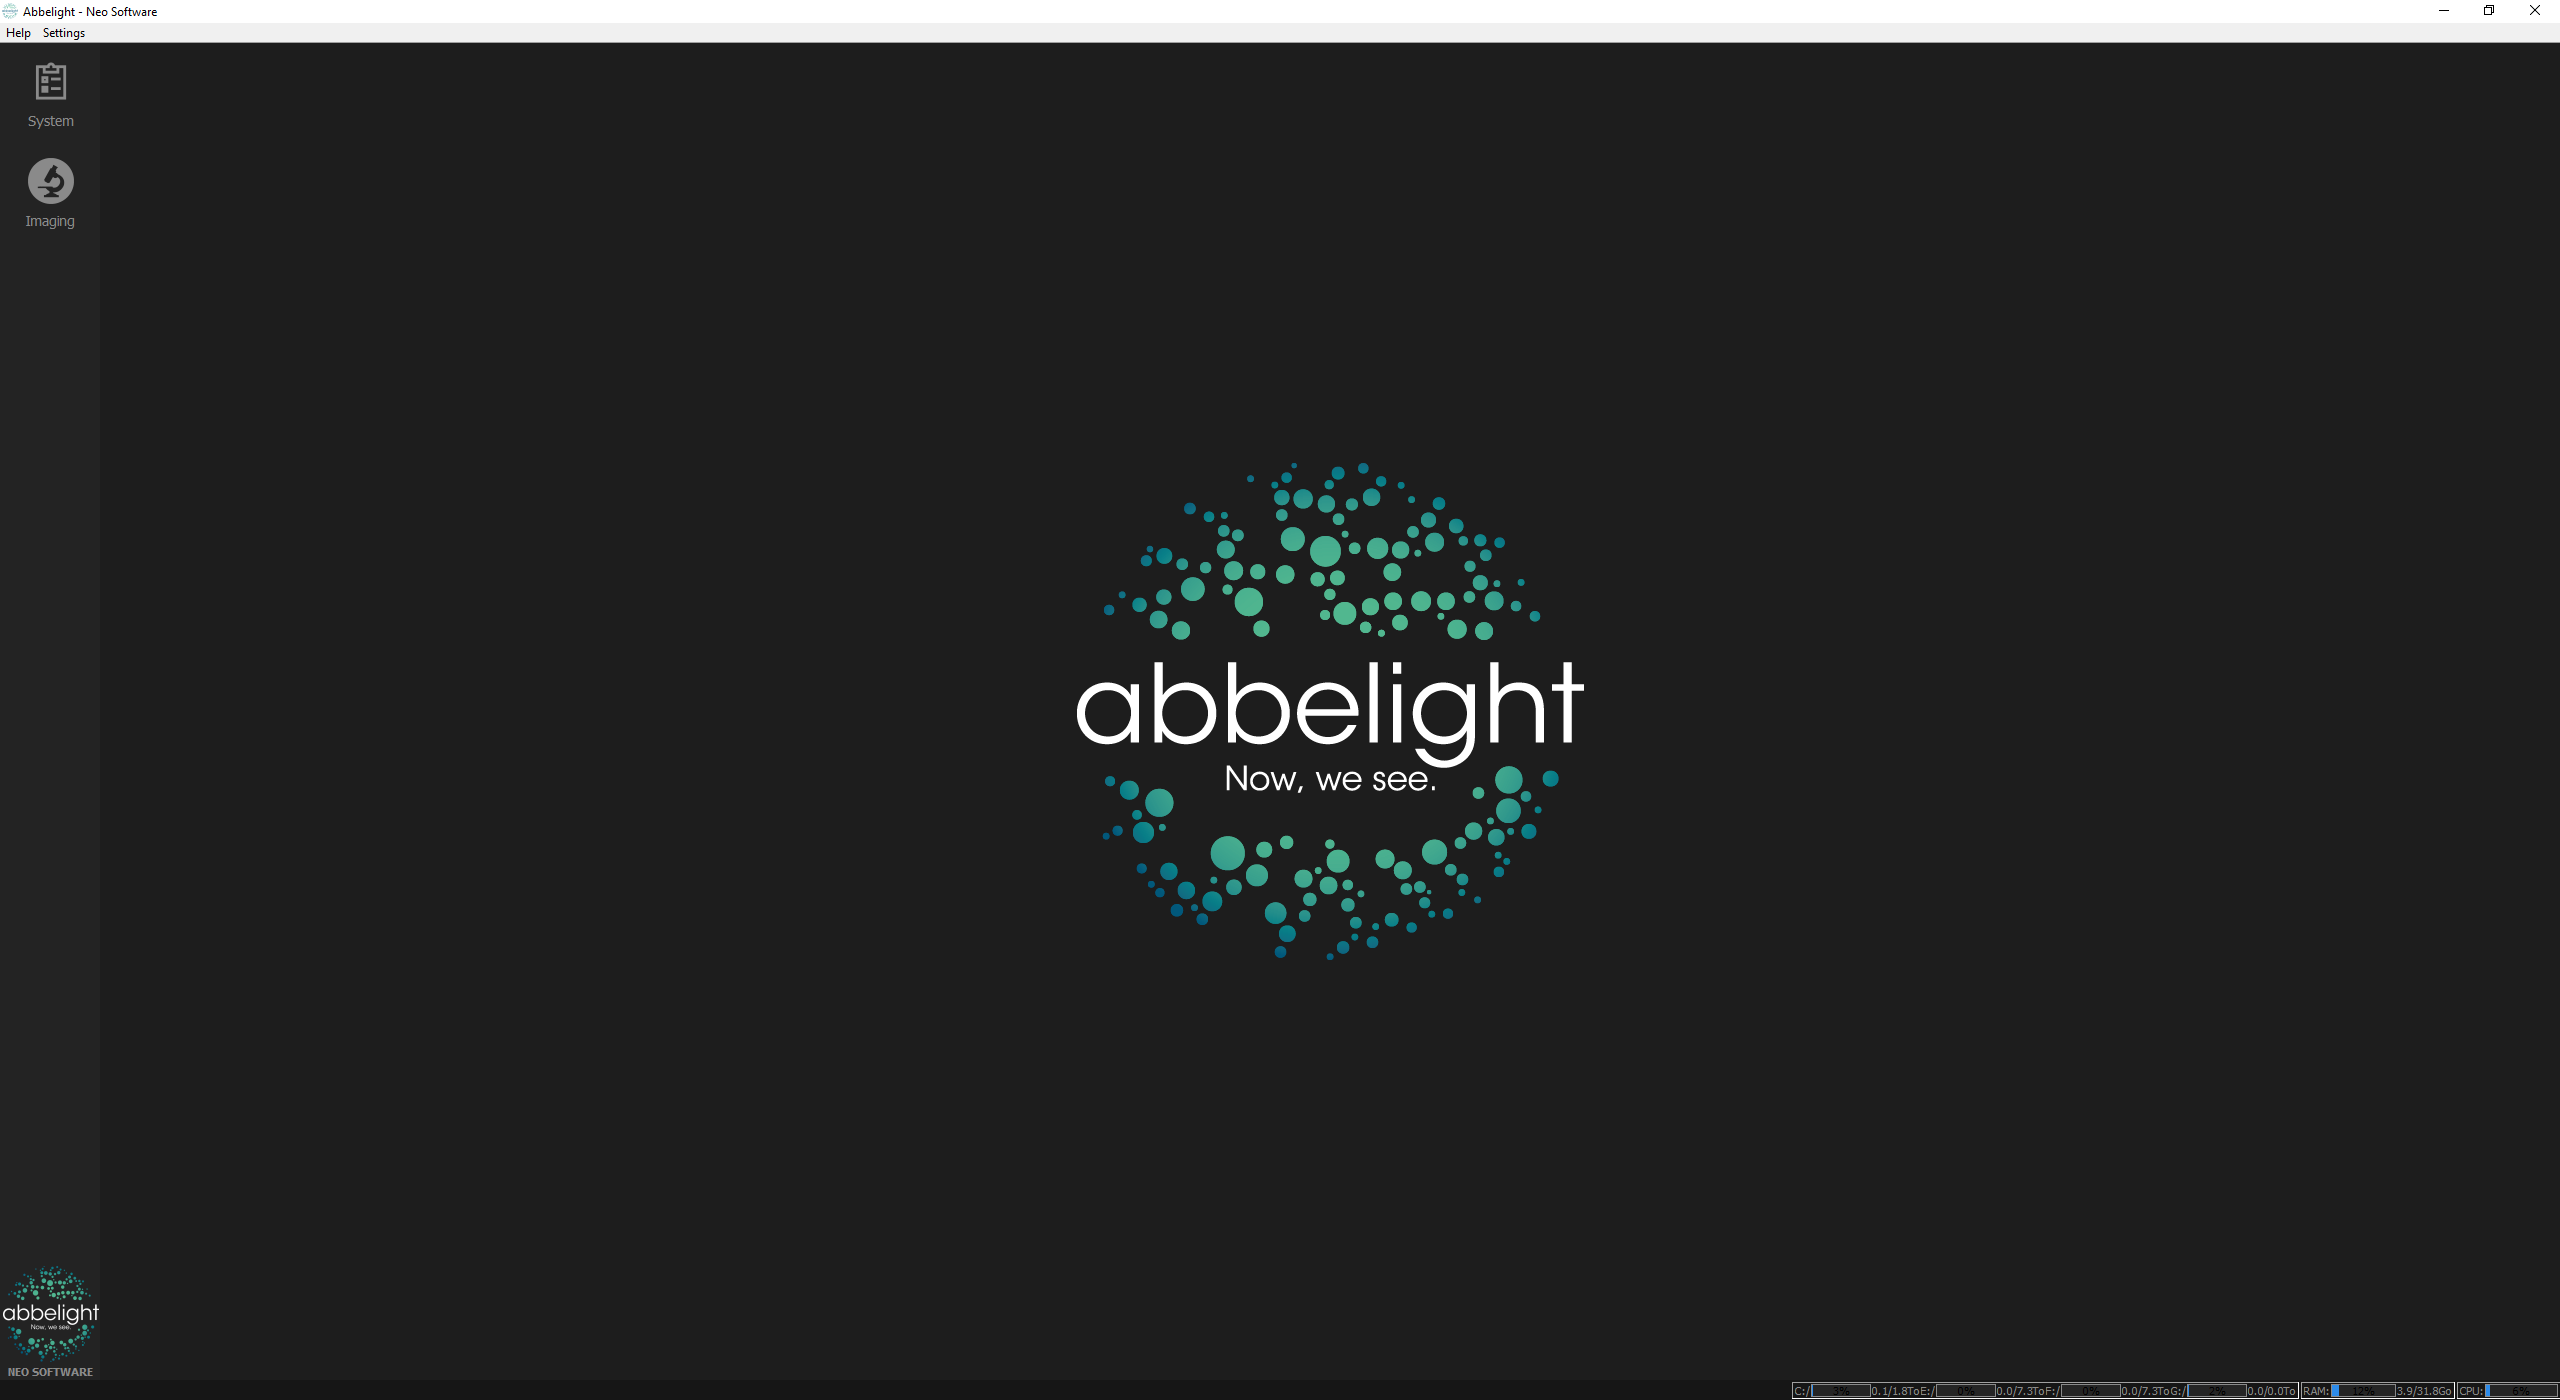
\includegraphics[width=0.75\textwidth]{liveimaging-startup.png}
    \caption{The NEO Live Imaging screen immediately after startup.}
    \label{fig:liveimaging-startup}
\end{figure}

From this screen, you can access two different modes of the software. The first is the `System' mode, which allows you to configure the microscope for different imaging modalities. The second mode is called `Imaging'. While in imaging mode, you directly control the invididual components of the microscope to acquire images.

Click `System'. You will see a screen like the one in \autoref{fig:liveimaging-system}. Clicking on `Hardware Configuration' will reveal a screen like \autoref{fig:liveimaging-hardware-config}. Ensure that the microscope is correct. It should be the `SAFe 180'. Also ensure that the resolution is set to `Nanoscopy' and that `2D' is selected. (3D imaging requires the insertion of an additional lens and a calibration step.) Finally, you can see the pixel size on the sample, which is the camera's physical pixel size divided by the magnification of the microscope. For a 100x objective, the pixel size should be about 108 nm.

\begin{figure}[ht]
    \centering
    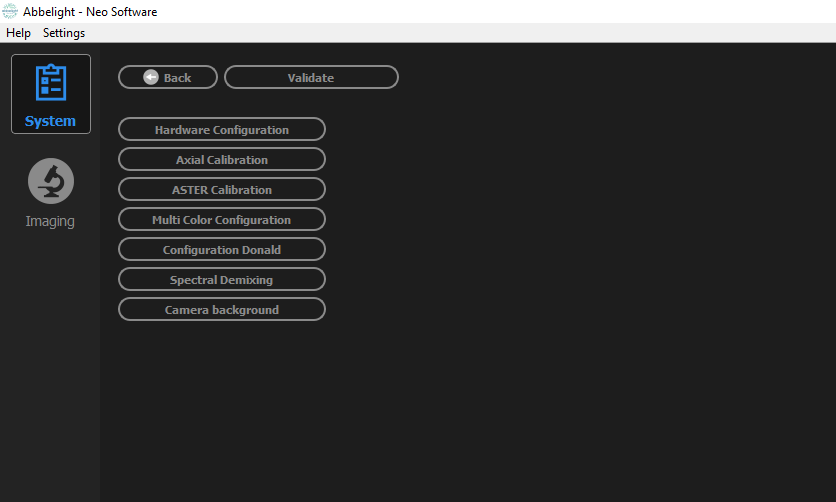
\includegraphics[width=1.0\textwidth]{liveimaging-system.png}
    \caption{The NEO Live Imaging screen in `System' mode.}
    \label{fig:liveimaging-system}
\end{figure}

\begin{figure}[ht]
    \centering
    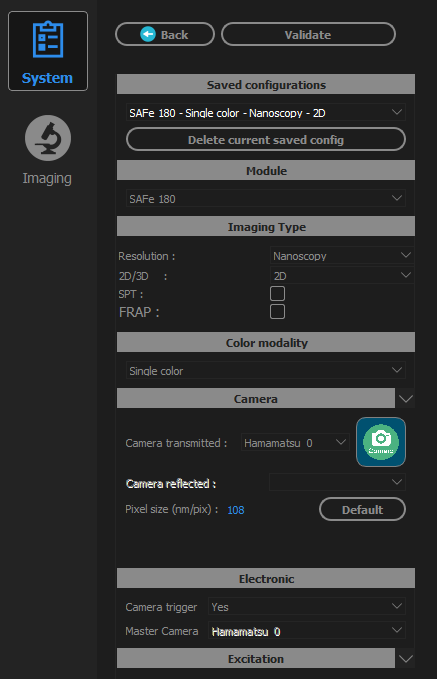
\includegraphics[height=0.5\textheight]{liveimaging-hardware-config.png}
    \caption{The NEO Live Imaging screen showing the current hardware configuration.}
    \label{fig:liveimaging-hardware-config}
\end{figure}

From this screen, you can also select the `Show Optical Path' button to see an illustration of the excitation and emission light paths through the microscope.

If everything looks good, click the `Back' button to go back to the `System' screen.

\subsubsection{Find the Sample}

\fbox{
    \parbox{\textwidth}{\textbf{TIP} It can help to turn off the room lights and close the window shades to reduce the amount of ambient light hitting the camera.}
}\newline

Now you will try to find the sample in the focal plane of the microscope. To start, click the `Imaging' button to put the microscope into imaging mode. Next, start a live stream from the camera by clicking the play button with the label `Start Preview'. You should now see a live image from the camera. The live stream will contain only noise.

Ensure that the metallic safety cover is in place over the objective and sample. If it is not, the lasers will not turn on. Turn on the red 642 nm laser by first selecting the `Settings' button to enable the laser controls. Then, toggle the radio button next to the \textbf{red} slider. Slide the slider a small amount to the right to increase the power slightly.

With the laser on, adjust the focus slowly to try and find the sample. You may need to increase the laser power a small amount and/or move the sample stage with the joystick. When the sample is in focus, you should see a clear image of the beads. This will look a little bit like a zoomed out view of \autoref{fig:fiji-bead-stack}, including many more beads over the larger field of view.

\subsubsection{Setup an Acquisition}

Here you are going to setup a time series acquisition of a field of view of beads. This will allow you to measure the 2D point spread function (PSF) of the microscope and the localization precision by repeatedly computing estimates for the bead positions and widths.

To setup a new acquisition, first create a project by clicking the `New Project' button. You will be prompted to enter a name for the project, as well as a path to the project data. The path should be \textbf{Documents/acquisition/YYYY-MM-DD-NAME1-NAME2} where `YYYY-MM-DD' are the year, month, and day of the acquisition. `NAME1' and `NAME2' are you and your partner's last names. Once finished, click `OK'. You will see the project appear in the project explorer pane. For the moment, there are no files in the project.

Next, start a live preview. Increase the red laser power until the beads are visible. In the `Settings' window, adjust the exposure time and the number of frames. Common values are 50 ms exporsures and 100 frames. Also ensure that `EPI' (epi-illumination) is selected for the illumination mode.

For the next step, double click in the window containing the live stream. This will create a green box to define a region of interest, or ROI. The area inside the ROI will be acquired during the acquisition.

Good ROI sizes are between $25 \, \mu m\times 25 \, \mu m$ and $100 \, \mu m\times 100 \, \mu m$, which is enough to cover several beads.

At this point, everything is set. Click the `Start' button to begin the acquisition. The acquisiton should take only a few seconds. When the acquisition is finished, you will see new files appear in the project explorer pane for this acquisition.

\subsection{Analysis}

\subsubsection{Measure the PSF Width and Localization Precision}

You will use the image analysis software FIJI to analyze the image data. Begin by opening FIJI. Then, open the file `ROI.tif' from the acquisition you just performed. You will see an image like the one in \autoref{fig:fiji-bead-stack}. If the image appears too dark, adjust the contrast by navigating to "Image \textgreater Adjust \textgreater Brightness/Contrast..." in the menu bar. Adjust the contrast by clicking the `Auto' button in the toolbar or by manually changing the minimum and maximum values.

\begin{figure}[ht]
    \centering
    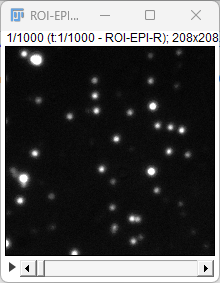
\includegraphics[width=0.5\textwidth]{fiji-bead-stack.png}
    \caption{A stack of images of fluorescent beads. The slider allows you to move through the stack, which in this example is moving through time.}
    \label{fig:fiji-bead-stack}
\end{figure}

Find a single, well-isolated fluorescent bead. We will use this bead to estimate the microscope PSF. First select the \textbf{Rectangle} tool from the FIJI toolbar. Click and drag a region around the bead. Select "Image \textgreater Crop" from the menu bar to crop the image to the region that you just selected. This will make working with the image easier.

Next, select the line tool from the toolbar as shown in \autoref{fig:fiji-line-tool}. Click and drag a line across the bead. (If you hold the Shift key while dragging, then you can ensure that the profile is perfectly horizontal or vertical.) The line should be long enough to cover the entire bead. Select "Analyze \textgreater Plot Profile" from the menu bar to plot the intensity profile of the bead. You should see a plot like the one in \autoref{fig:fiji-plot-profile}. The plot shows the intensity of the bead along the line that you drew. The peak of the plot corresponds to the \textbf{approximate} center of the bead. The width of the peak corresponds to the width of the PSF.

\begin{figure}[ht]
    \centering
    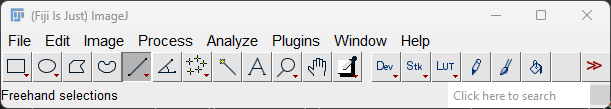
\includegraphics[width=0.75\textwidth]{fiji-line-tool.png}
    \caption{The line tool selected in FIJI.}
    \label{fig:fiji-line-tool}
\end{figure}

\begin{figure}[ht]
    \centering
    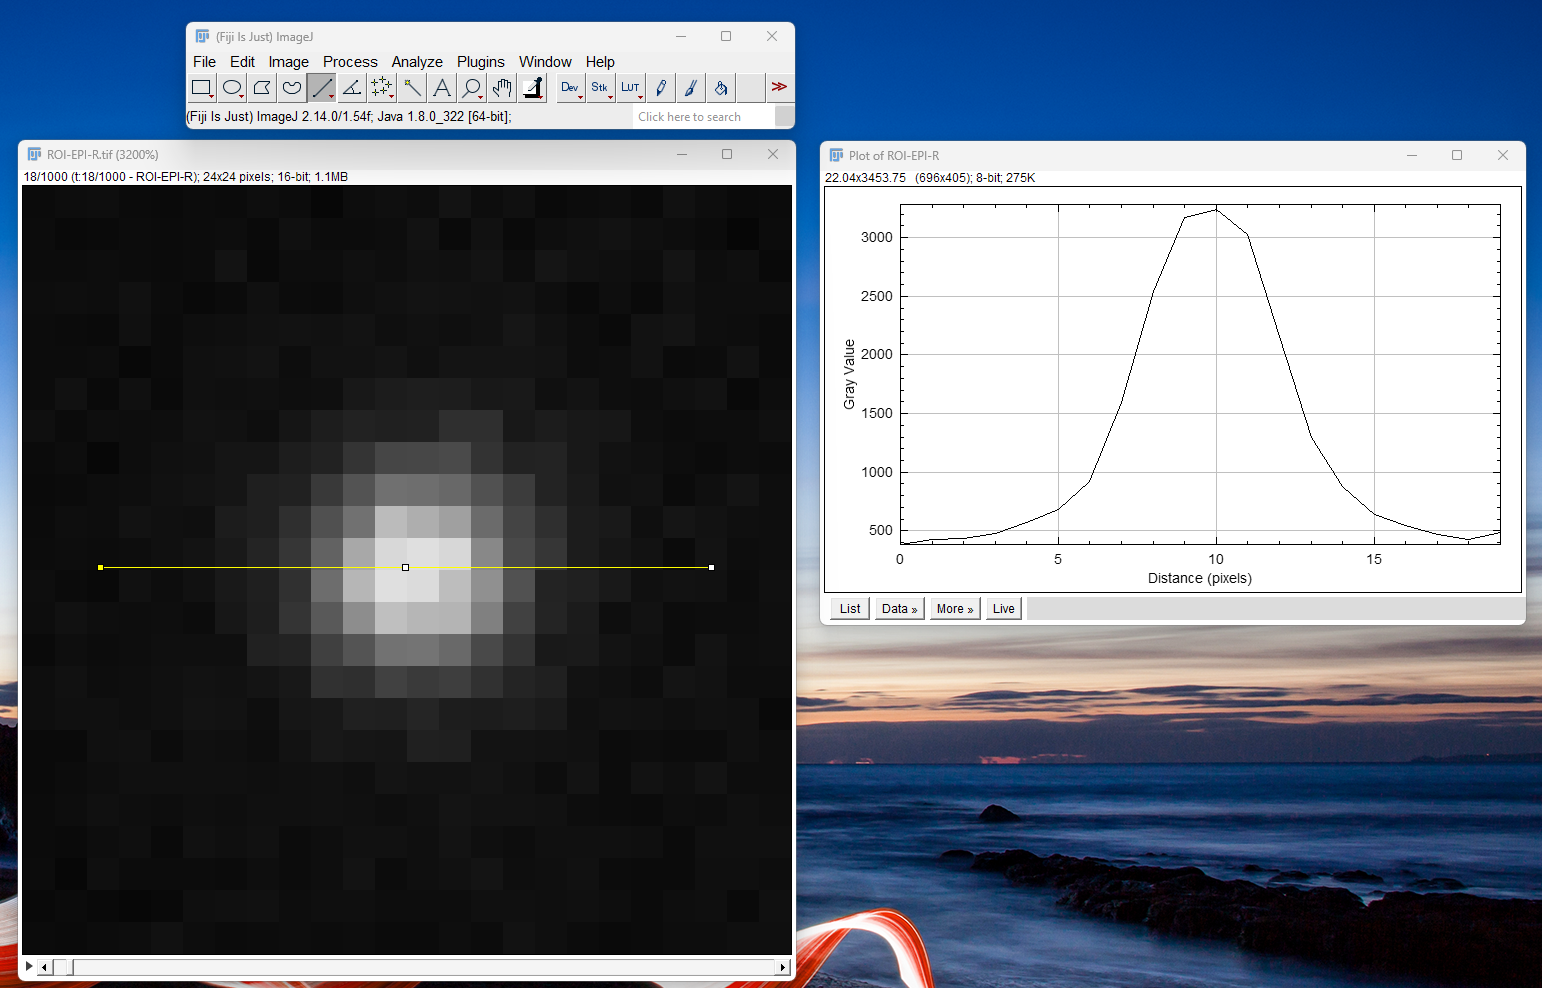
\includegraphics[width=0.9\textwidth]{fiji-plot-profile.png}
    \caption{The intensity profile of a bead.}
    \label{fig:fiji-plot-profile}
\end{figure}

Click "Live" in the line profile window so that you can observe changes to the profile in real time. Double click the line tool and increase the width of the line to cover the bead. This will look like \autoref{fig:fiji-plot-profile-thick}. In this mode, the profile is computed by averaging the pixel intensities in directions perpendicular to the line. Doing so helps remove the effects of noise.

\begin{figure}[ht]
    \centering
    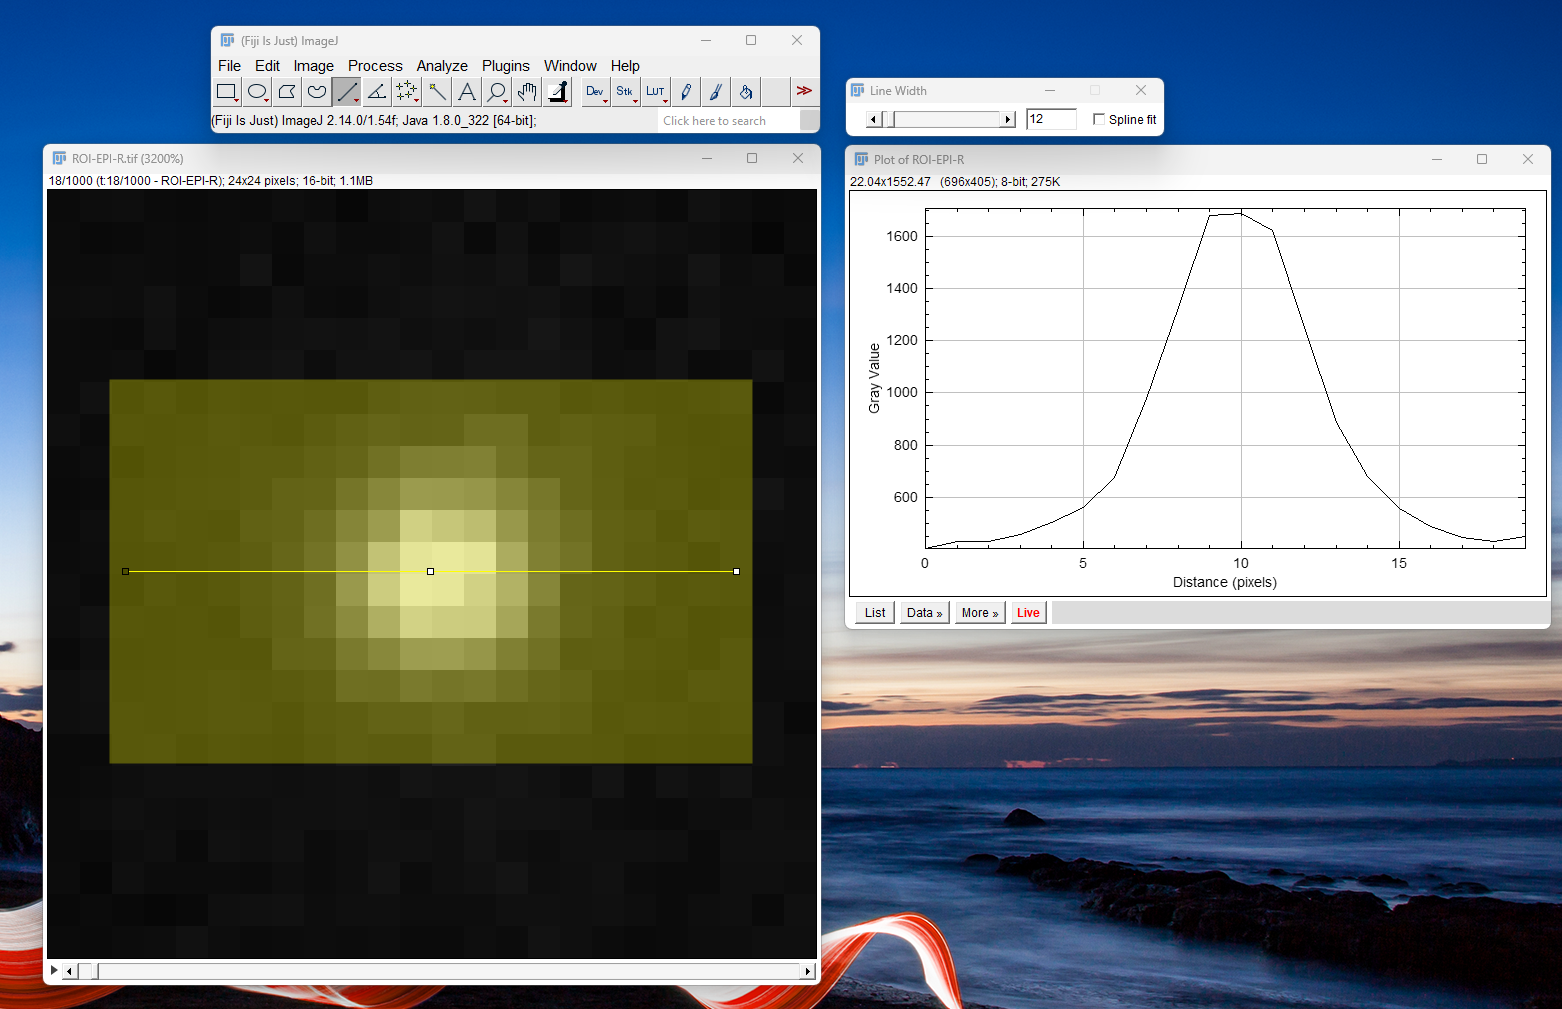
\includegraphics[width=0.9\textwidth]{fiji-plot-profile-thick.png}
    \caption{The intensity profile of a bead with a thick line.}
    \label{fig:fiji-plot-profile-thick}
\end{figure}

If we only take the peak of the curve as the bead's position, then we are limited to a precision of one pixel. We can do better by fitting a model of the PSF to the profile. The simplest model for the PSF is a Gaussian curve.\footnote{Remember that the Airy disk is a better model, but the Gaussian is good enough in many cases and simpler to work with.} To fit a Gaussian to the profile, select the "Data \textgreater \textgreater" button in the Plot Profile window and choose "Select Fit..." from the popup menu. Select "Gaussian" from the fit function menu. After clicking OK, should see the best-fit Gaussian curve overlaid on the data, as well as a table of the fit parameters. The fit parameters are the mean, standard deviation, and amplitude of the Gaussian curve. The mean is the position bead, and the standard deviation is the width of the curve.

Note that almost certainly the bead position will be in fractions of a pixel, meaning that you have located the bead center with sub-pixel accuracy.

Record the fit parameters for both the mean of the Gaussian and the standard deviation from at least ten frames. (You automate the procedure to do more if you wish.)

Repeat this procedure for other laser wavelengths. In total, you should use the 488 nm laser, the 561 nm laser, and the 647 nm laser.

\subsubsection{Questions and Tasks: Experiment 1}

You should answer the following questions in your final report:

\begin{enumerate}
    \item What is the width of the PSF as determined from the images of beads and how does it compare to theory? Remember that theory states that the distance between the center of the PSF and first zero is $dr = 0.61 \lambda / \text{NA}$.
    \item From the bead images, determine the localization precision by fitting a Gaussian curve to images of single fluorescent beads and making histograms of the x and y positions. How does the uncertainty in the localization precision depend on the number of photons collected?
\end{enumerate}

Include the following plots in your report:

\begin{enumerate}
    \item A histogram or scatterplot of the fitted Gaussian PSF widths with the mean and standard deviation indicated. This represents the PSF width and uncertainty.
    \item A plot of PSF width vs. wavelength.
    \item A histogram or scatterplot of the fitted Gaussian positions with the mean and standard deviation indicated. This represents the localization precision and uncertainty.
\end{enumerate}

\section{Experiment 2 - STORM Imaging of Microtubules}\label{sec:exp2}

In this experiment you will take images of blinking, fluorescent molecules attached to the microtubules in COS7 cells. From the movies of blinking molecules you will reconstruct a super-resolved image of the microtubule network.

\begin{figure}[ht]
    \centering
    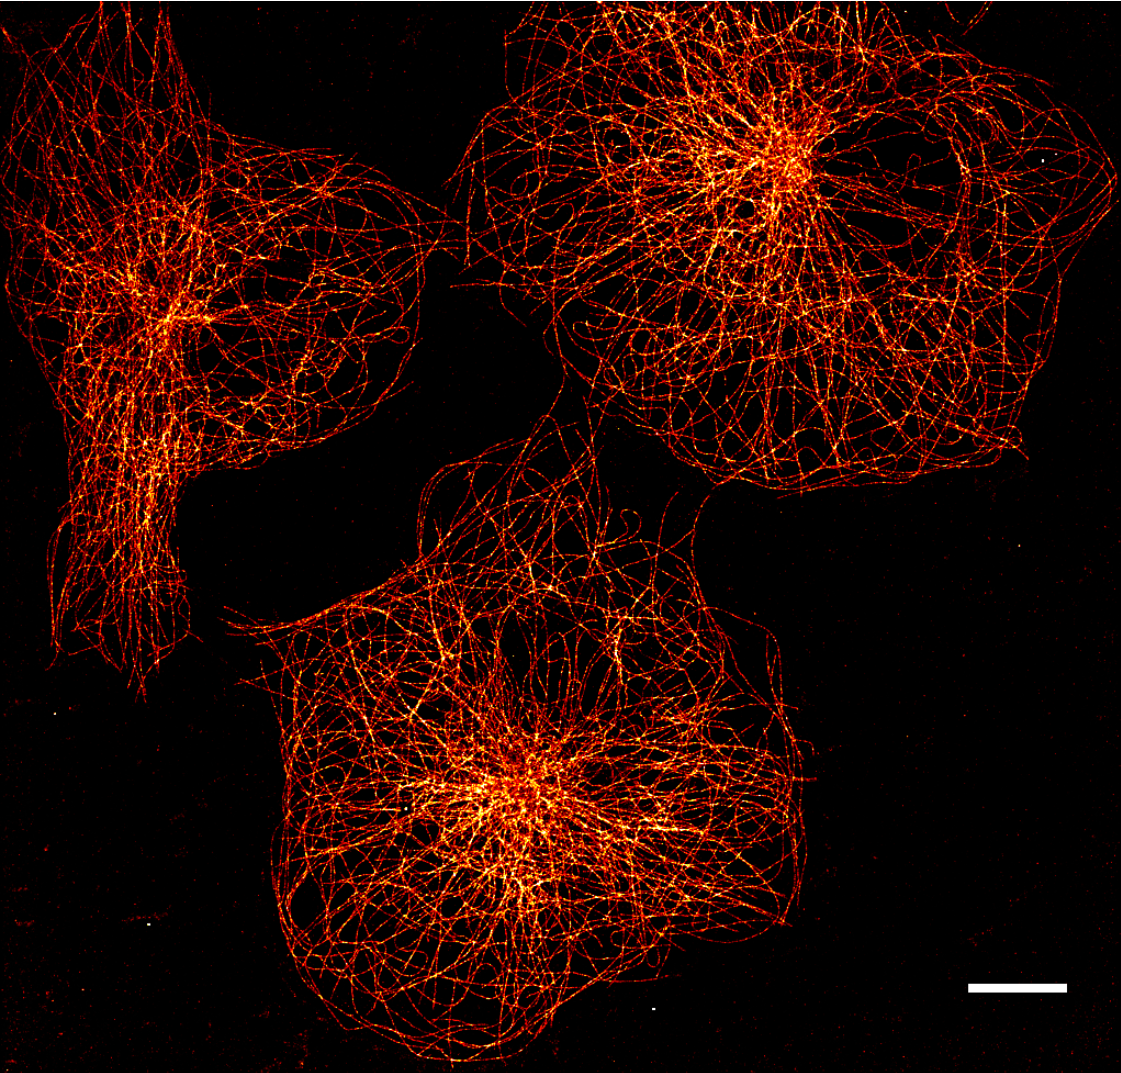
\includegraphics[width=0.75\textwidth]{cos7-microtubules.png}
    \caption{STORM image of microtubules in COS7 cells. Cells were labelled with antibodies against $\alpha$-tubulin and secondary antibodies conjugated with AlexaFluor 647. Scale bar 10 $\mu$m. From \cite{douglass-naturephotonics-2016}.}
    \label{fig:cos7-microtubules}
\end{figure}

\subsection{Materials}

\begin{itemize}
    \item{Mounted cell sample (see \autoref{sec:mount-sample})}
    \item{Immersion oil}
    \item{Lens cleaning products (see \autoref{sec:remove-oil})}
\end{itemize}

\subsection{Procedure}

\subsubsection{Mount the Sample}\label{sec:mount-sample}

For STORM imaging you will need to mount the coverslips onto a slide with buffer. The sample is mounted in two steps: 1. mount the sample coverslip onto a glass cavity well slide, and 2. mount the slide/coverslip combination onto the microscope.

\subsubsection{Mount the Coverslip onto the Slide}

\fbox{
    \parbox{\textwidth}{\textbf{WARNING} Gloves and eye protection must be worn for this procedure.}
}\newline

A video tutorial describing this process may be found at \url{https://drive.google.com/file/d/1czRAzCVn1dEPEgESOuVnm_-1_1xvhQnW/view?usp=sharing}. You need to be signed in with your EPFL account to view the video.

Mounting the coverslip onto the slide requires the following materials:

\begin{itemize}
    \item{Glass cavity well slide}
    \item{Coverslip with sample}
    \item{Buffer kit}
    \item{Picodent sealant (both yellow and blue components)}
    \item{Tweezers}
    \item{Pipettes}
    \item{10 $\mu$L and 1 mL pipette tips}
    \item{Paper towels}
\end{itemize}

Begin by mixing the components of the buffer kit. Add 10 $\mu$L of solution from the green tube the blue tube. \textbf{Be sure to never exceed the soft stop on the pipette because you may accidentally suck solution into it.} Mix the solution by pipetting it up and down several times. Next, add 6 $\mu$L of solution from the red tube to blue tube. Mix the solution again. The buffer is now ready to use.

For the next step, load 175 $\mu$L of the prepared buffer solution into the cavity slide using a 1 mL pipette tip. Then, using tweezers, gently pick up the coverslip with the cell sample on it and place it over the cavity well with the sample side facing into the buffer. Gently remove any excess buffer by placing a paper towel over the slide.

If there is a bubble, \textbf{very gently} slide the coverslip to the side until the bubble is exposed. Add a tiny bit more buffer, then slide the coverslip back to the center of the well. Remove any excess buffer as before.

Finally, mix together equal amounts of the Picodent sealant's yellow and blue components in a small dish with a 1 mL pipette tip. When properly mixed, the sealant will turn to a light green color. Using the same tip, add the sealant around the entirety of the coverslip edge to prevent any buffer from leaking out.

\subsubsection{Find the Sample}

This part is largely the same as in the beginning of the procedure of \autoref{sec:exp1} where you found the sample.

With the laser on and at low power, adjust the focus slowly to try and find the sample. You may need to increase the laser power a small amount and/or move the sample stage with the joystick. When the sample is in focus, you should see a clear image of the cells. Out-of-focus images will appear blurry, as in \autoref{fig:in-vs-out-of-focus}. If, after several minutes, you are unable to find the sample, ask for help. It could be that the cells have detached from the coverslip, in which case you would need to mount a new sample.

\begin{figure}[ht]
    \centering
    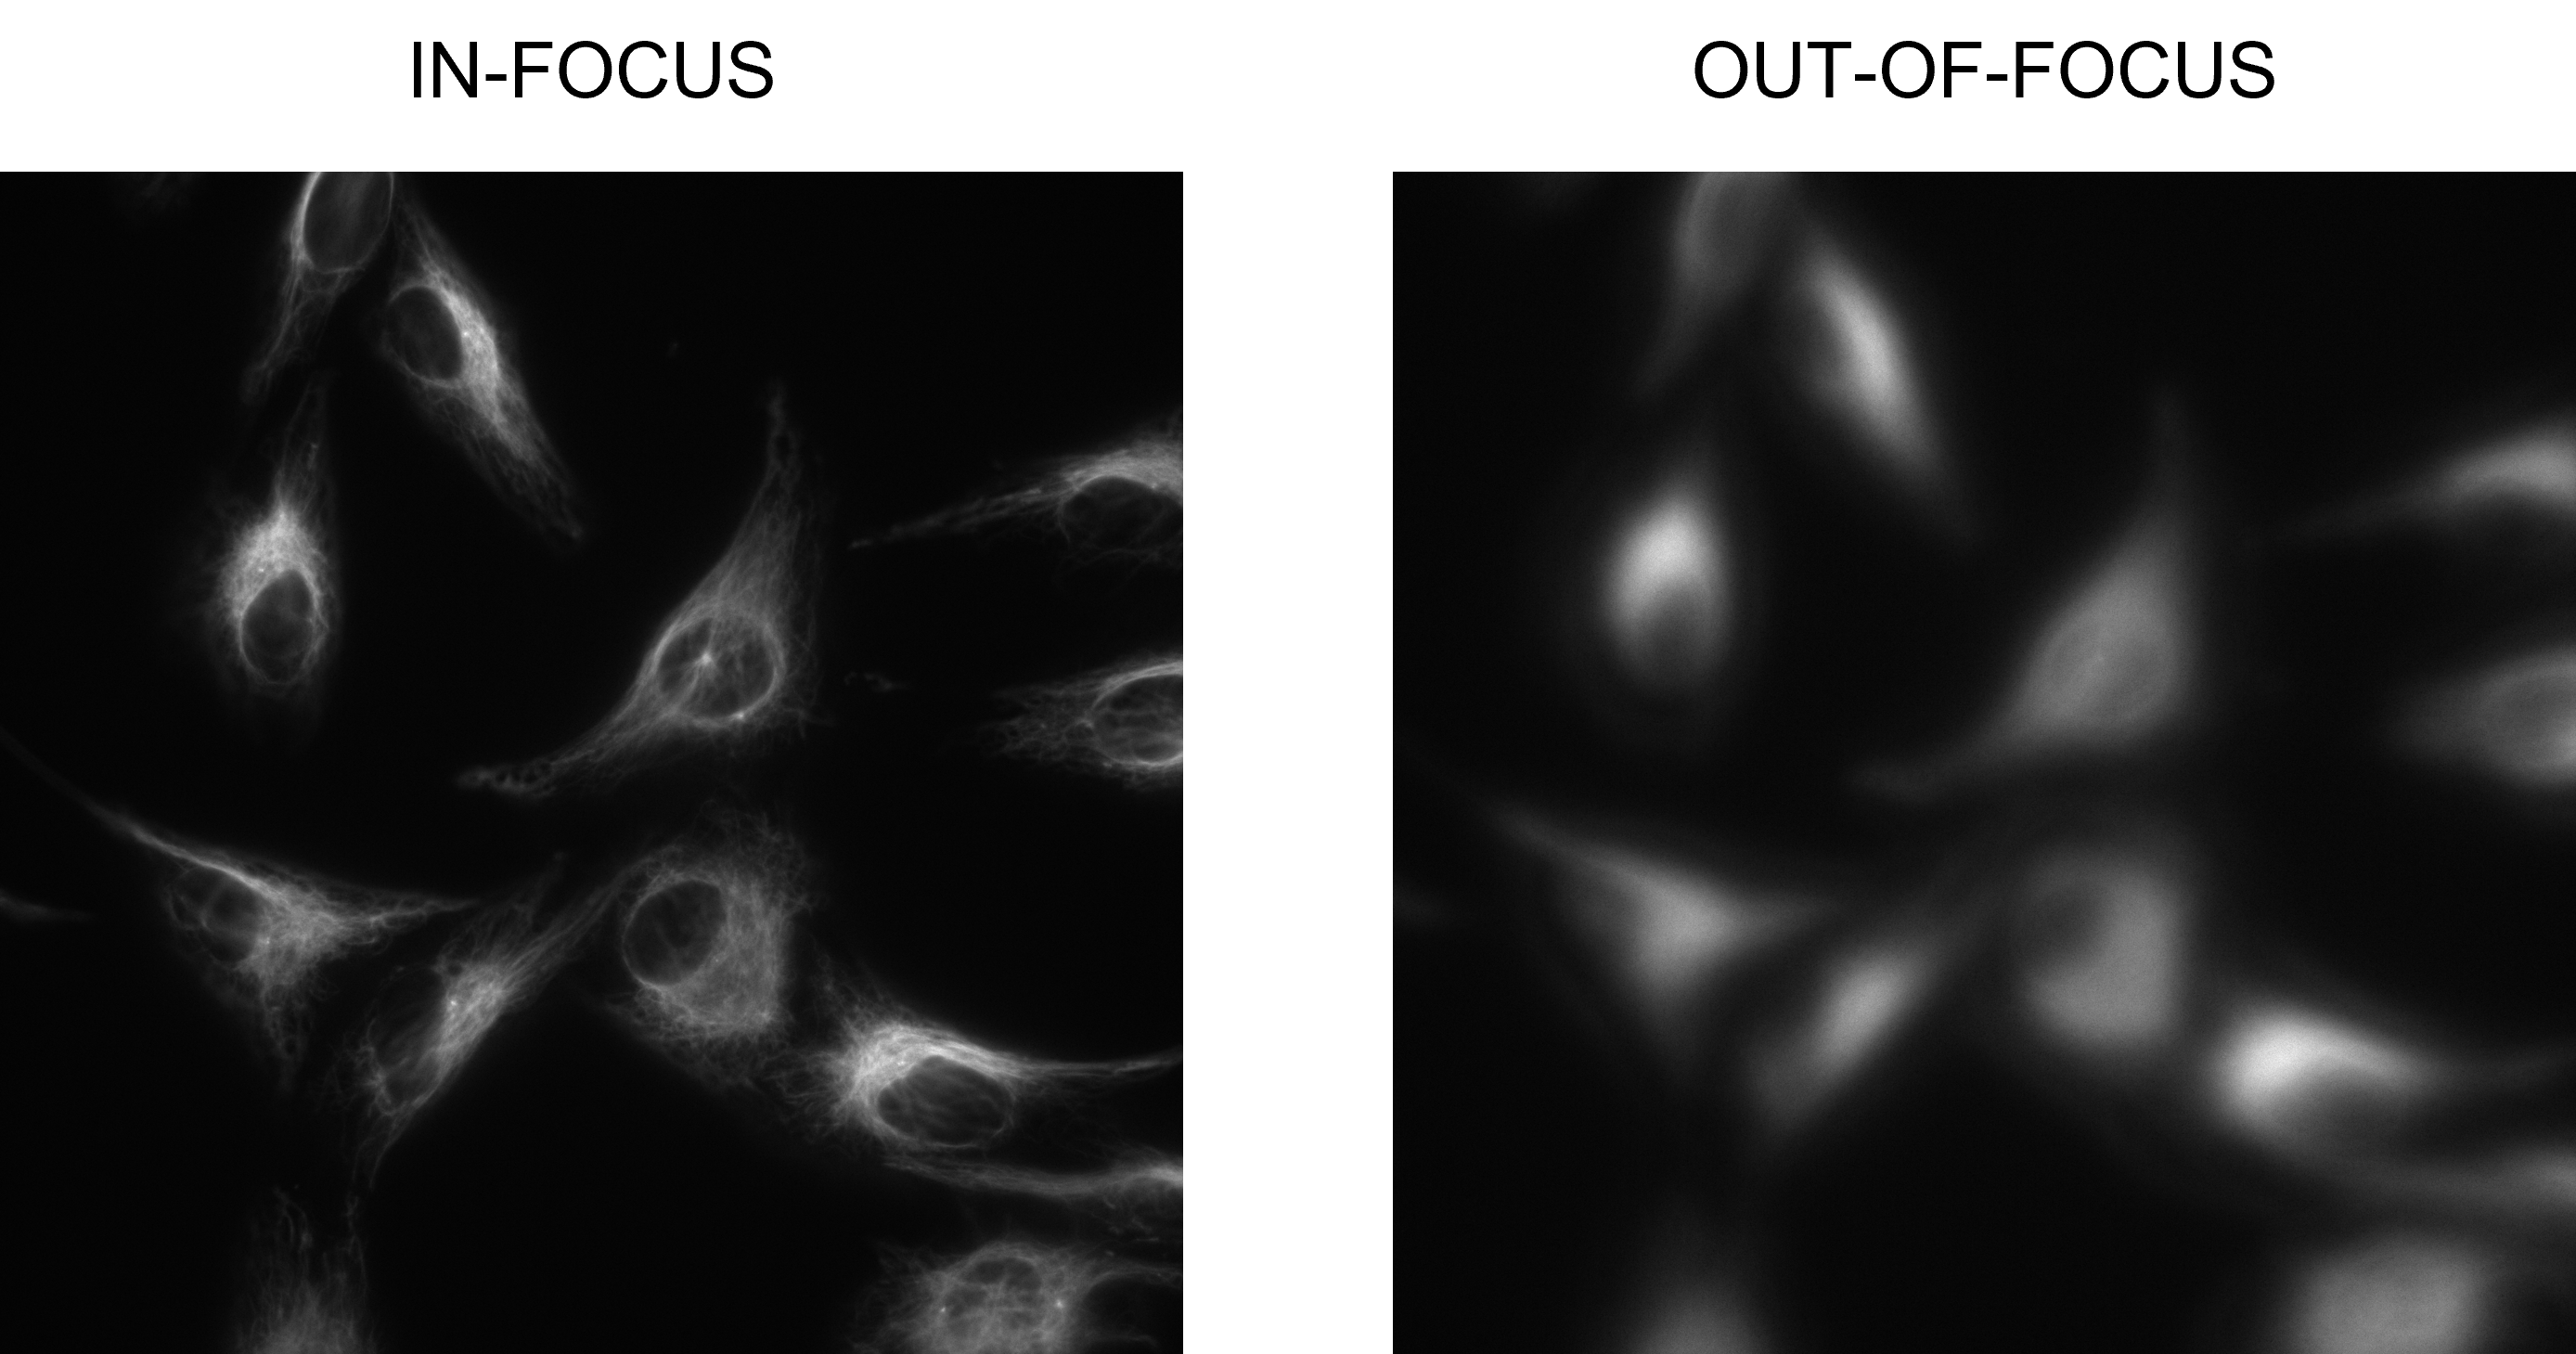
\includegraphics[width=1.0\textwidth]{in-vs-out-of-focus.png}
    \caption{An in-focus image of microtubules in COS7 cells (left) and an out-of-focus image (right). Images courtesy of Matt Lycas.}
    \label{fig:in-vs-out-of-focus}
\end{figure}

\subsubsection{Setup a STORM Acquisition}

A STORM acquisiton is a series of frames recorded from the sample in which the fluorophores are blinking on and off. To setup a new acquisition, first create a project by clicking the `New Project' button. You will be prompted to enter a name for the project, as well as a path to the project data. The path should be \textbf{Documents/acquisition/YYYY-MM-DD-NAME1-NAME2} where `YYYY-MM-DD' are the year, month, and day of the acquisition. `NAME1' and `NAME2' are you and your partner's last names. Once finished, click `OK'. You will see the project appear in the project explorer pane. For the moment, there are no files in the project.

Next, start a live preview. Increase the red laser power until the fluorescent molecules start to blink on and off rapidly. Try to set the power so that there are no overlapping images of individual fluorescent molecules in any one frame. In the `Settings' window, adjust the exposure time and the number of frames. Common values are 50 ms exporsures and 10,000 frames. Also ensure that `EPI' (epi-illumination) is selected for the illumination mode. The settings will look similar to those in \autoref{fig:liveimaging-imaging-settings}.

\begin{figure}[ht]
    \centering
    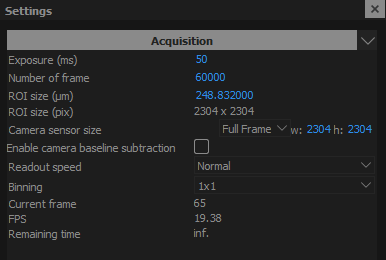
\includegraphics[width=0.75\textwidth]{liveimaging-imaging-settings.png}
    \caption{The NEO Live Imaging screen showing the default acquisition settings. Note the exposure time and the number of frames.}
    \label{fig:liveimaging-imaging-settings}
\end{figure}

For the next step, double click in the window containing the live stream. This will create a green box to define a region of interest, or ROI. The area inside the ROI will be acquired during the acquisition.

\fbox{
    \parbox{\textwidth}{\textbf{TIP} Always use a ROI for STORM imaging. Using the full camera frame will create very large datasets that are difficult to work with.}
}\newline

Good ROI sizes are between $25 \, \mu m\times 25 \, \mu m$ and $100 \, \mu m\times 100 \, \mu m$, which is large enough to cover about one cell.

The final thing to do before starting the acquisition is to engage the autofocus system. Autofocus is a mechanism that maintains the focus on the sample by measuring an infrared light source that is reflected from the coverslip. During imaging, very small temperature changes can cause the focus to drift. Focal drift can ruin SMLM images because different frames from an acquisition will be focused on different parts of the sample. To engage the autofocus (after you have found the focus), click the \textbf{Continuous AF} tab on the microscope controller box, and then click the \textbf{Start} button. You should disengage it when you are not acquiring.

At this point, everything is set. Click the `Start' button to begin the acquisition. At 50 ms and 10,000 frames, an acquisiton will take about 8 minutes. You can see how many frames have been acquired in the settings pane. When the acquisition is finished, you will see new files appear in the project explorer pane for this acquisition.

\subsubsection{Tune the Density of Emitters}

During the acquisition, you will need to maintain a good density of emitters. A good density is one where the single molecule images do not overlap and where at least one fluoresecent molecule per PSF area is emitting light. \autoref{fig:good-vs-bad-density} shows examples of good and bad emitter densities.

\begin{figure}[ht]
    \centering
    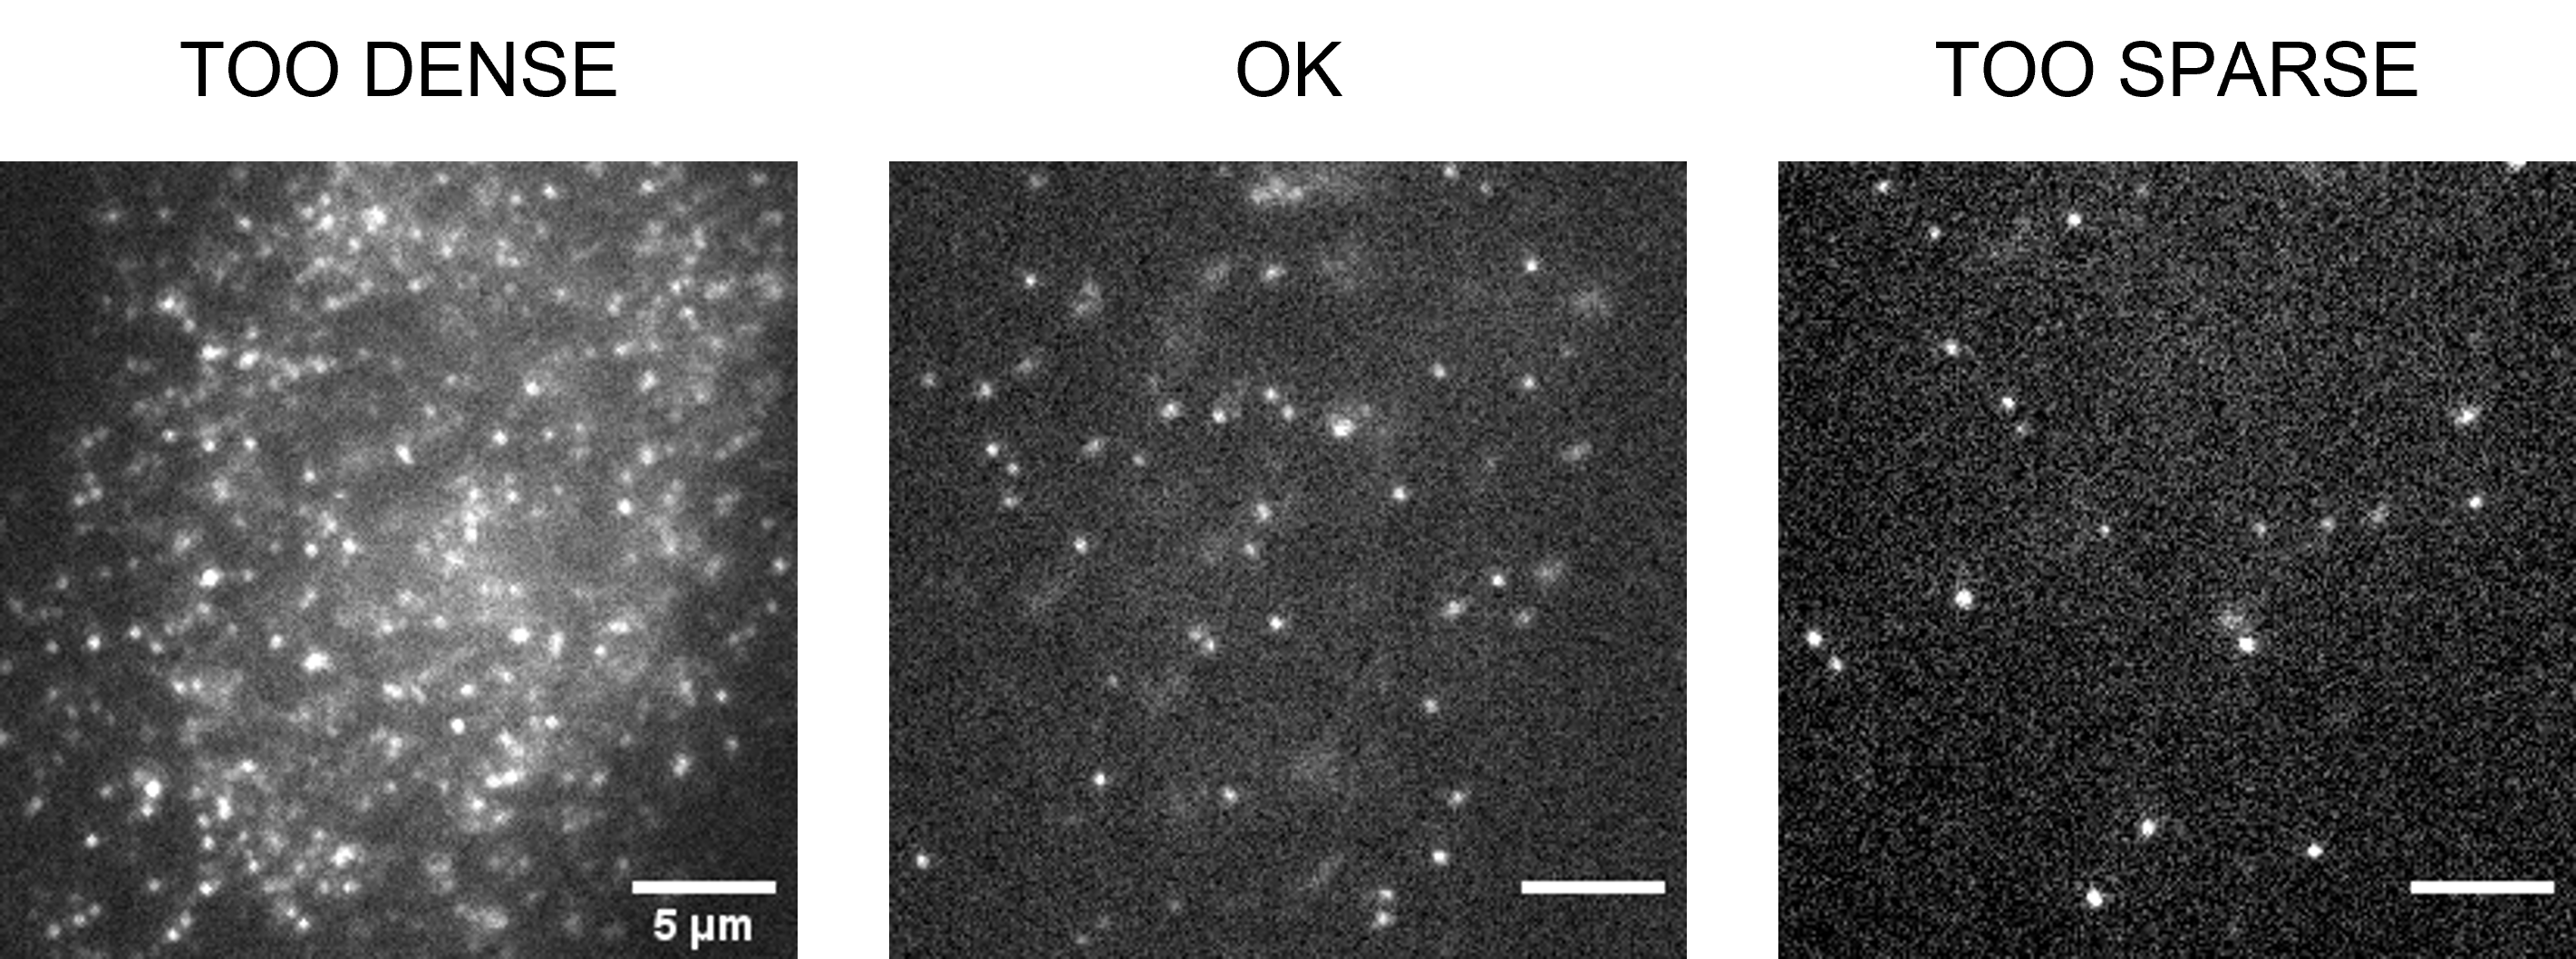
\includegraphics[width=1.0\textwidth]{sm-density-examples.png}
    \caption{Examples of too dense, good, and too sparse densities of fluorescent emitters. These are single frames from a STORM acquisition of nucleoporins on the nuclear membrane of U2OS cells.}
    \label{fig:good-vs-bad-density}
\end{figure}

Movies of the blinking fluorophores can be found at the following links:

\begin{itemize}
    \item \href{https://drive.google.com/file/d/12zIK-BqMl0qttkYljKi7P9xZ3krMvthe/view?usp=sharing}{Too Dense}
    \item \href{https://drive.google.com/file/d/1Is4U-K297sku4u20OJqwY6IOUags1bLl/view?usp=sharing}{Good}
    \item \href{https://drive.google.com/file/d/1W2AxVjYirPj8t8d2__m8rNoNTUyM3RfY/view?usp=sharing}{Too Sparse}
\end{itemize}

To maintain a good density of emitters, you will need to adjust the laser power during the acquisition. If the density is too high, you can either increase the amount of 642 nm (red) laser power, or decrease the amount of 405 nm (UV) laser power (if you are using any). If the density is too low, you can either decrease the amount of 642 nm laser power, or increase the amount of 405 nm laser power. You can also adjust the exposure time to increase or decrease the number of photons collected per frame, but this cannot be set once an acquisiton has started.

Try to acquire enough images that you can answer the questions in \autoref{sec:questions}.

\subsubsection{Clean up}

\fbox{
    \parbox{\textwidth}{\textbf{WARNING} Gloves and eye protection must be worn for this procedure. Do not let the buffer touch your skin.}
}\newline

When you are done acquiring data, clean up the microscope objective as described in \autoref{sec:remove-oil}.

Also, remove any oil from the sample slide. To do this, use lens cleaning solution and lens tissue. Once done, you can slide a pair of tweezers underneath the picodent sealant to remove the coverslip and place it back in PBS. Dispose of the slide in the glass waste bin, and any excess buffer in the buffer waste.

\subsection{Analysis}

\subsubsection{Compute the Localizations}

In the previous section you acquired image stacks of blinking single molecules. In this section, you will reconstruct a super-resolution image from the raw data.

To begin, open the software called \textbf{NEO Analysis}. Click on the `Batch' button to enter batch processing mode. Here you will configure which files to process and how to process them. Select `Input Dataset', which will open a File Open... dialog window. Navigate to one of your datasets and select the `ROI.tif' file from within the dataset. This file contains the raw image stack that will be processed into a single super-resolution image. For now, leave all the options at their default values for processing.

Now, you can either add another dataset to process by selecting `Add Dataset', or start the analysis by clicking the `Start' button.

Processing can take several minutes, or even more than an hour if many large datasets are being processed. \autoref{fig:smlm-data-analysis} illustrates the procedure. During processing, images of single fluorescent molecules will first be filtered. This will facilitate identification of the images of single fluorescent molecules. Peak finding algorithms will then be run on the filtered images to segment them into indiviual square regions. Next, the positions of the molecules will be determined to precisions on the order of $\approx 10 \, nm$ by fitting point spread function (PSF) models to them. Finally, the positions will be rendered into a super-resolution image. The localization results will be saved in the same directory as the raw data by default.

\begin{figure}
    \centering
    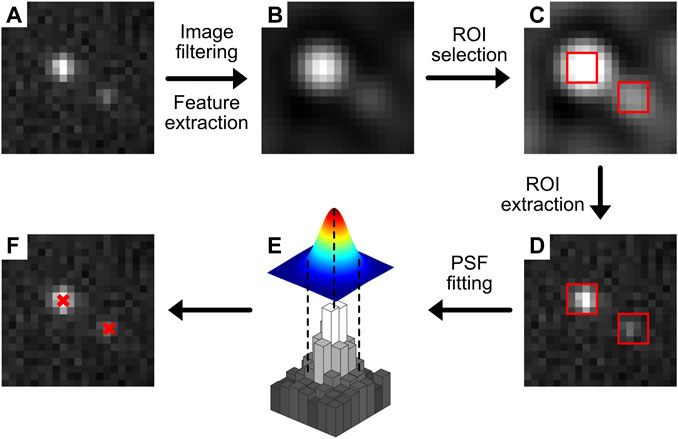
\includegraphics[width=1.0\textwidth]{smlm-data-analysis.jpg}
    \caption{The steps involved in processing raw data into a super-resolution image. Image from \cite{martens-frontiersinbioinformatics-2022}.}
    \label{fig:smlm-data-analysis}
\end{figure}

\subsubsection{Visualize the Localizations}

The final steps that remain involve analyzing the localization data and super-resolution image. Click `Batch' to exit Batch mode, and then click `3D Viewer' to open the 3D viewer. Then click `Load File' to select a file containing localization data from the previous steps. These files will be named `CoordTable\_SAFE180\_2D.csv'. After loading the file, you will see a 3D rendering of the localizations. From here you can attempt filtering and further processing on the localizations.

See \autoref{sec:questions} for more information about what to try during these post-processing steps. For a more complete discussion of the many ways to analyze super-resolution data, please see \cite{martens-frontiersinbioinformatics-2022}.

\section{Experiment 3 - STORM Imaging of Mitochondria}\label{sec:exp3}

\begin{figure}[ht]
    \centering
    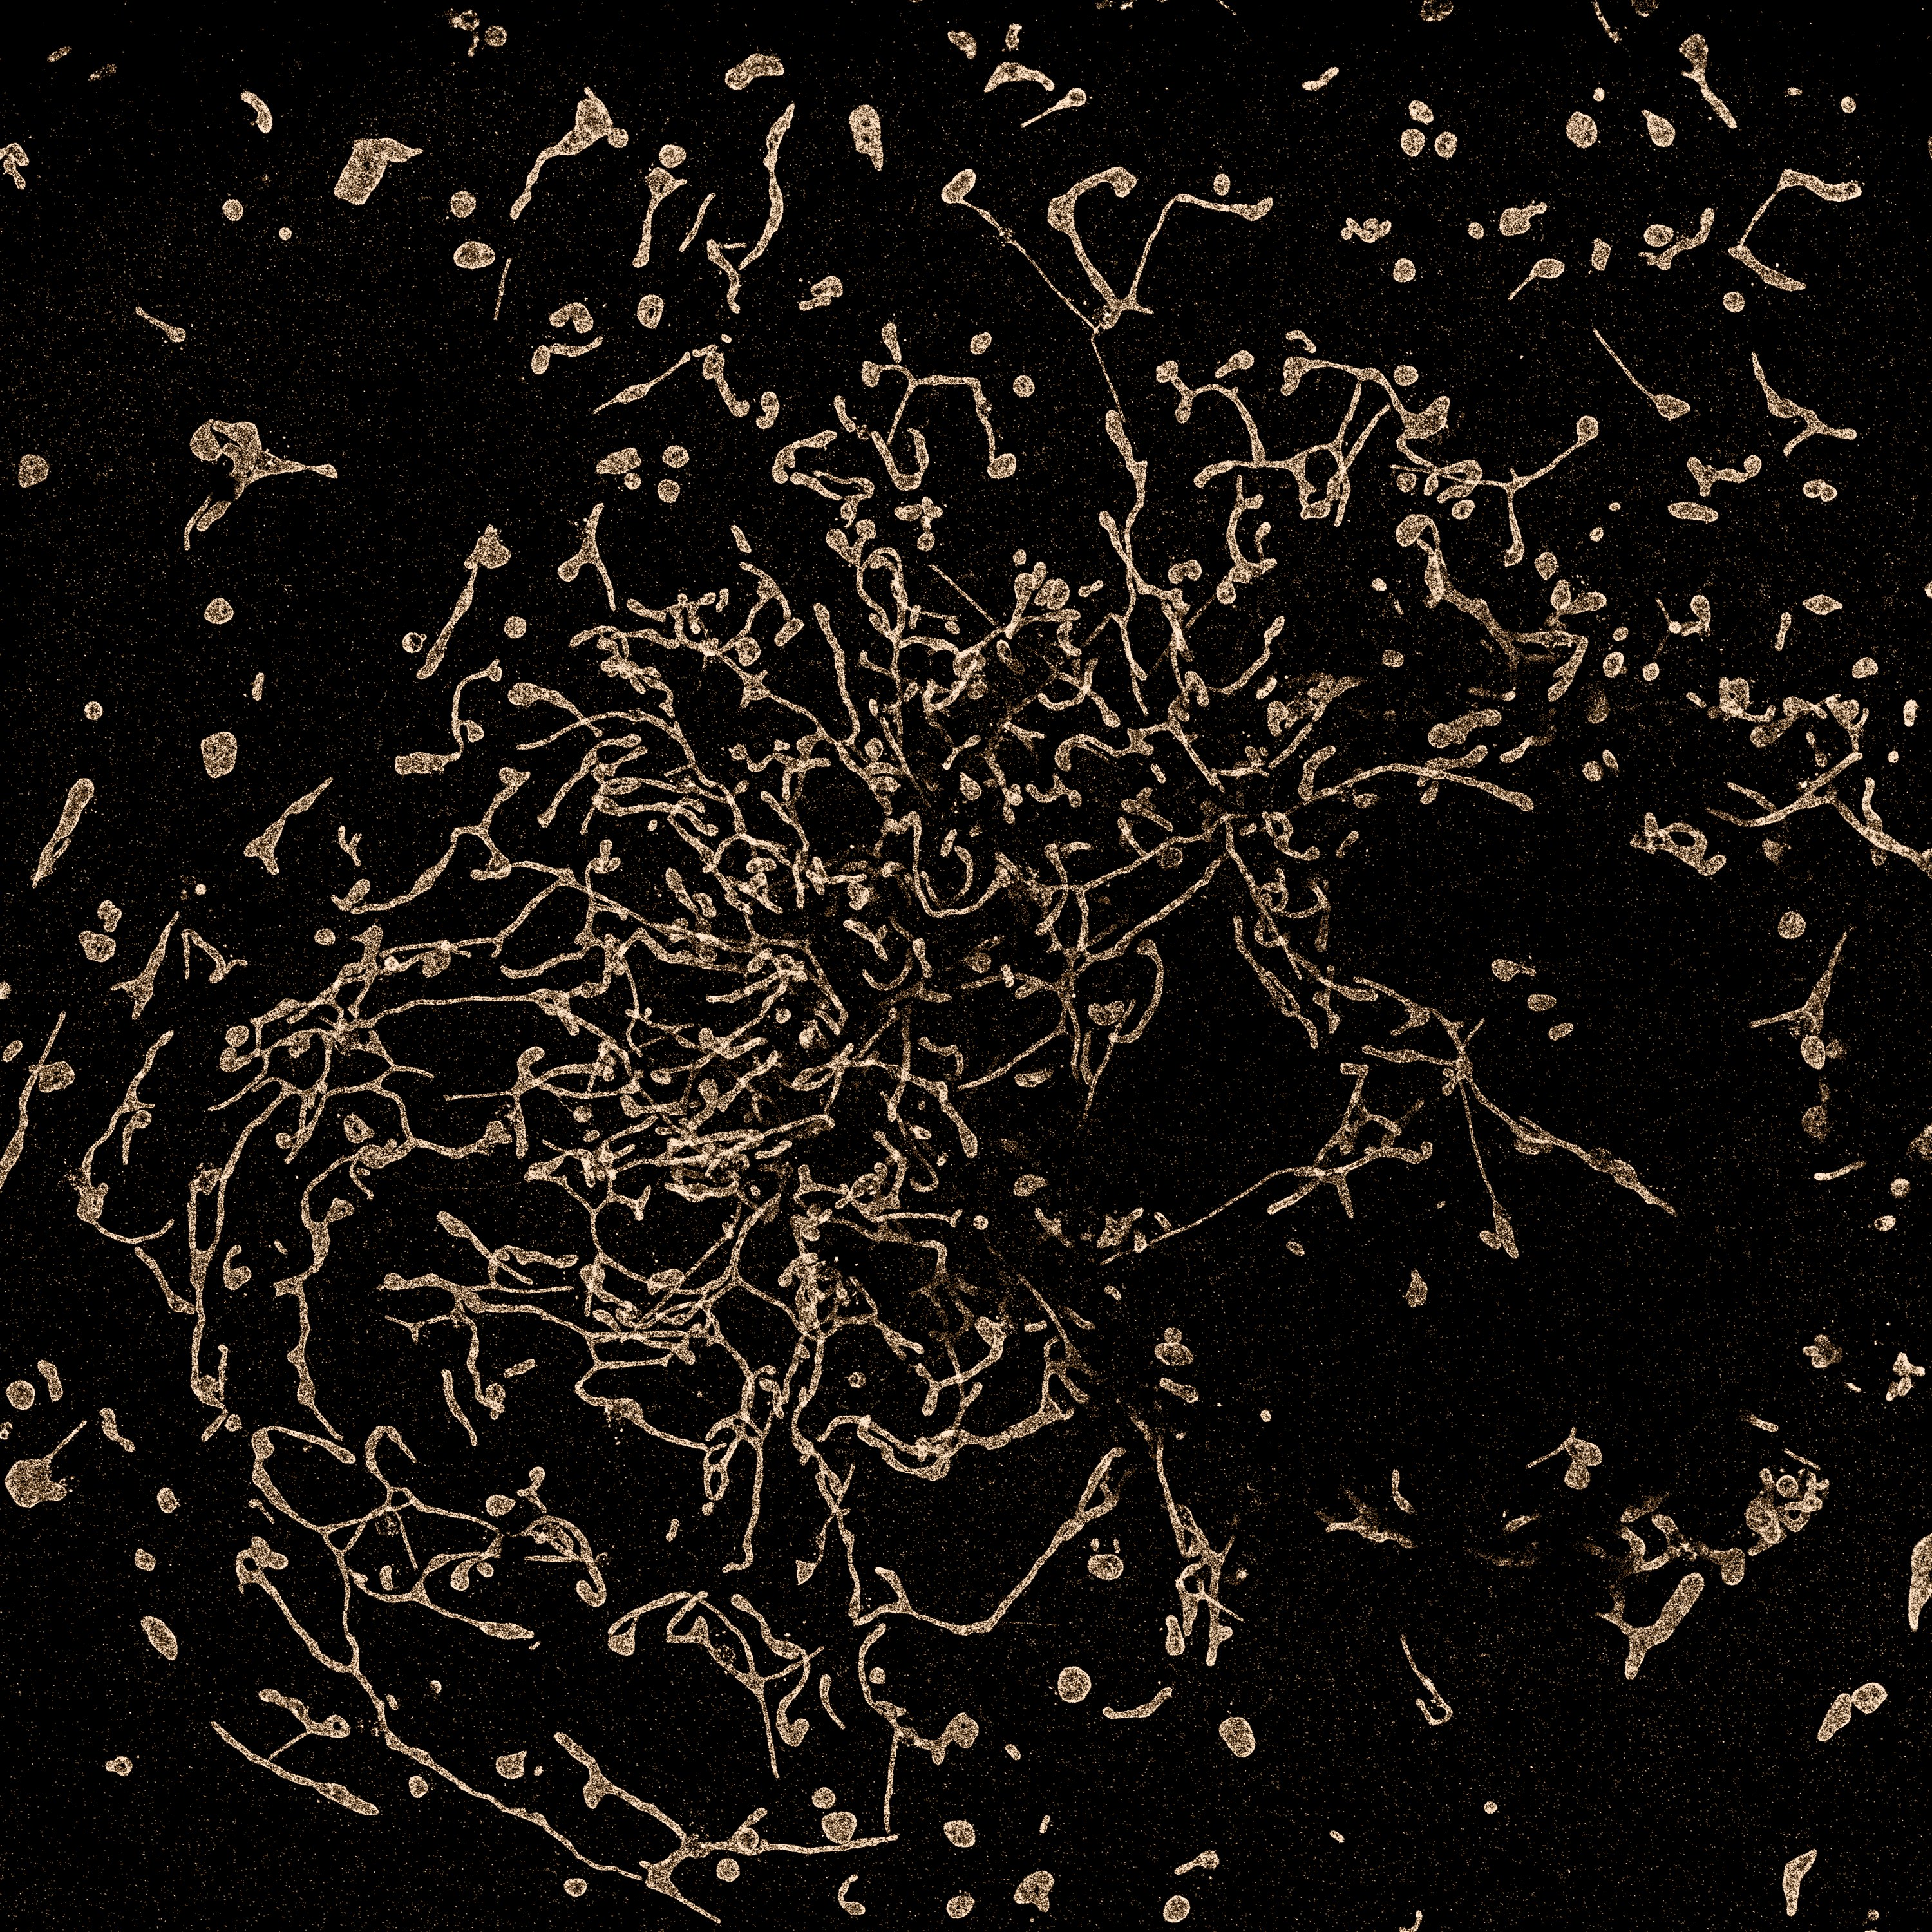
\includegraphics[width=0.75\textwidth]{cos7-mitochondria.jpeg}
    \caption{STORM image of mitochondria in COS7 cells.}
    \label{fig:cos7-mitochondria}
\end{figure}

This experiment is performed exactly as in \autoref{sec:exp2}, except that the mitochondrial sample is used.

\subsection{Questions: Experiments 2 and 3}\label{sec:questions}

The following analyses should be included in your final report:

\begin{enumerate}
    \item What is the width of a microtubule as imaged in SMLM? Try to find the distance between the double peak as we discussed. If you did not manage to do this, discuss what it was that you think prevented you from doing it. If you did, manage, how does it compare to published values for the width as measured with STORM or PALM?
\end{enumerate}

In addition, you should answer the following questions based on what you learned during these experiments:

\begin{enumerate}
    \item{What is the difference between a STORM image and a conventional fluorescence image?}
    \item{What is the effect of the red (642 nm) laser power in STORM imaging?}
    \item{What is the effect of the UV (405 nm) laser power in STORM imaging?}
    \item{What is the effect of the exposure time in STORM imaging? What does it mean when the exposure time is too high or too low?}
    \item{What is the effect of changing the number of frames in a SMLM acquisition?}
    \item{Do you think drift correction is necessary to produce good images?}
    \item{Is it necessary to filter the localizations to get a good image, for example by removing localizations with bad values of uncertainty or goodness-of-fit paramters? Why or why not?}
    \item{What makes a good STORM image? How can you tell during an acquisiton whether the super-resolution image will be good or not?}
    \item{Which is easier to image: microtubules or mitochondria? Why?}
    \item{If you failed to create any super-resolution images, what do you think went wrong? What could be improved?}
\end{enumerate}

\end{document}
